\chapter{Experimental Setup and Testing}\label{ch:testing}\addtocontents{lof}{\protect\contentsline{chapter}{\protect\numberline{\thechapter}Experimental Setup and Testing}{}{}}
% \openepigraph{Everything in its right place \\
% There are two colours in my head}{Radiohead \textit{Everything In Its Right Place}}
\vspace{-2.5em}
% \newthought{Synopsis}\synopsisMethod

\mynewline
After completing the literature review I decided to go down two main paths: developing a representative valve and a anatomical valve. The representative valve would be a simple model that could be used to test the simulator and the anatomical valve would be a more complex model that could be used to test the simulator and also be used for educational purposes.

\section{Fixturing Assembly}
The assembly process began with seating the valve in it's ring holder and passing the chordae tendineae through the evenly spaced notches of the ring fixture.

The chordae tendineae were tensioned evenly by hanging the two part fixture in a retort stand and manually pulling the wires through the notch fixture until visibly evenly tensioned, at which point Buna-N rubber wedges were inserted to hold the tension in place.

The assembly fixturing being all one piece was inserted through the distal end of the polycarbonate tubing, once the end cap was press fit into the tubing a hook tool was used to manuver the seated valve into place further down the tube.


\begin{figure}
    \centering
    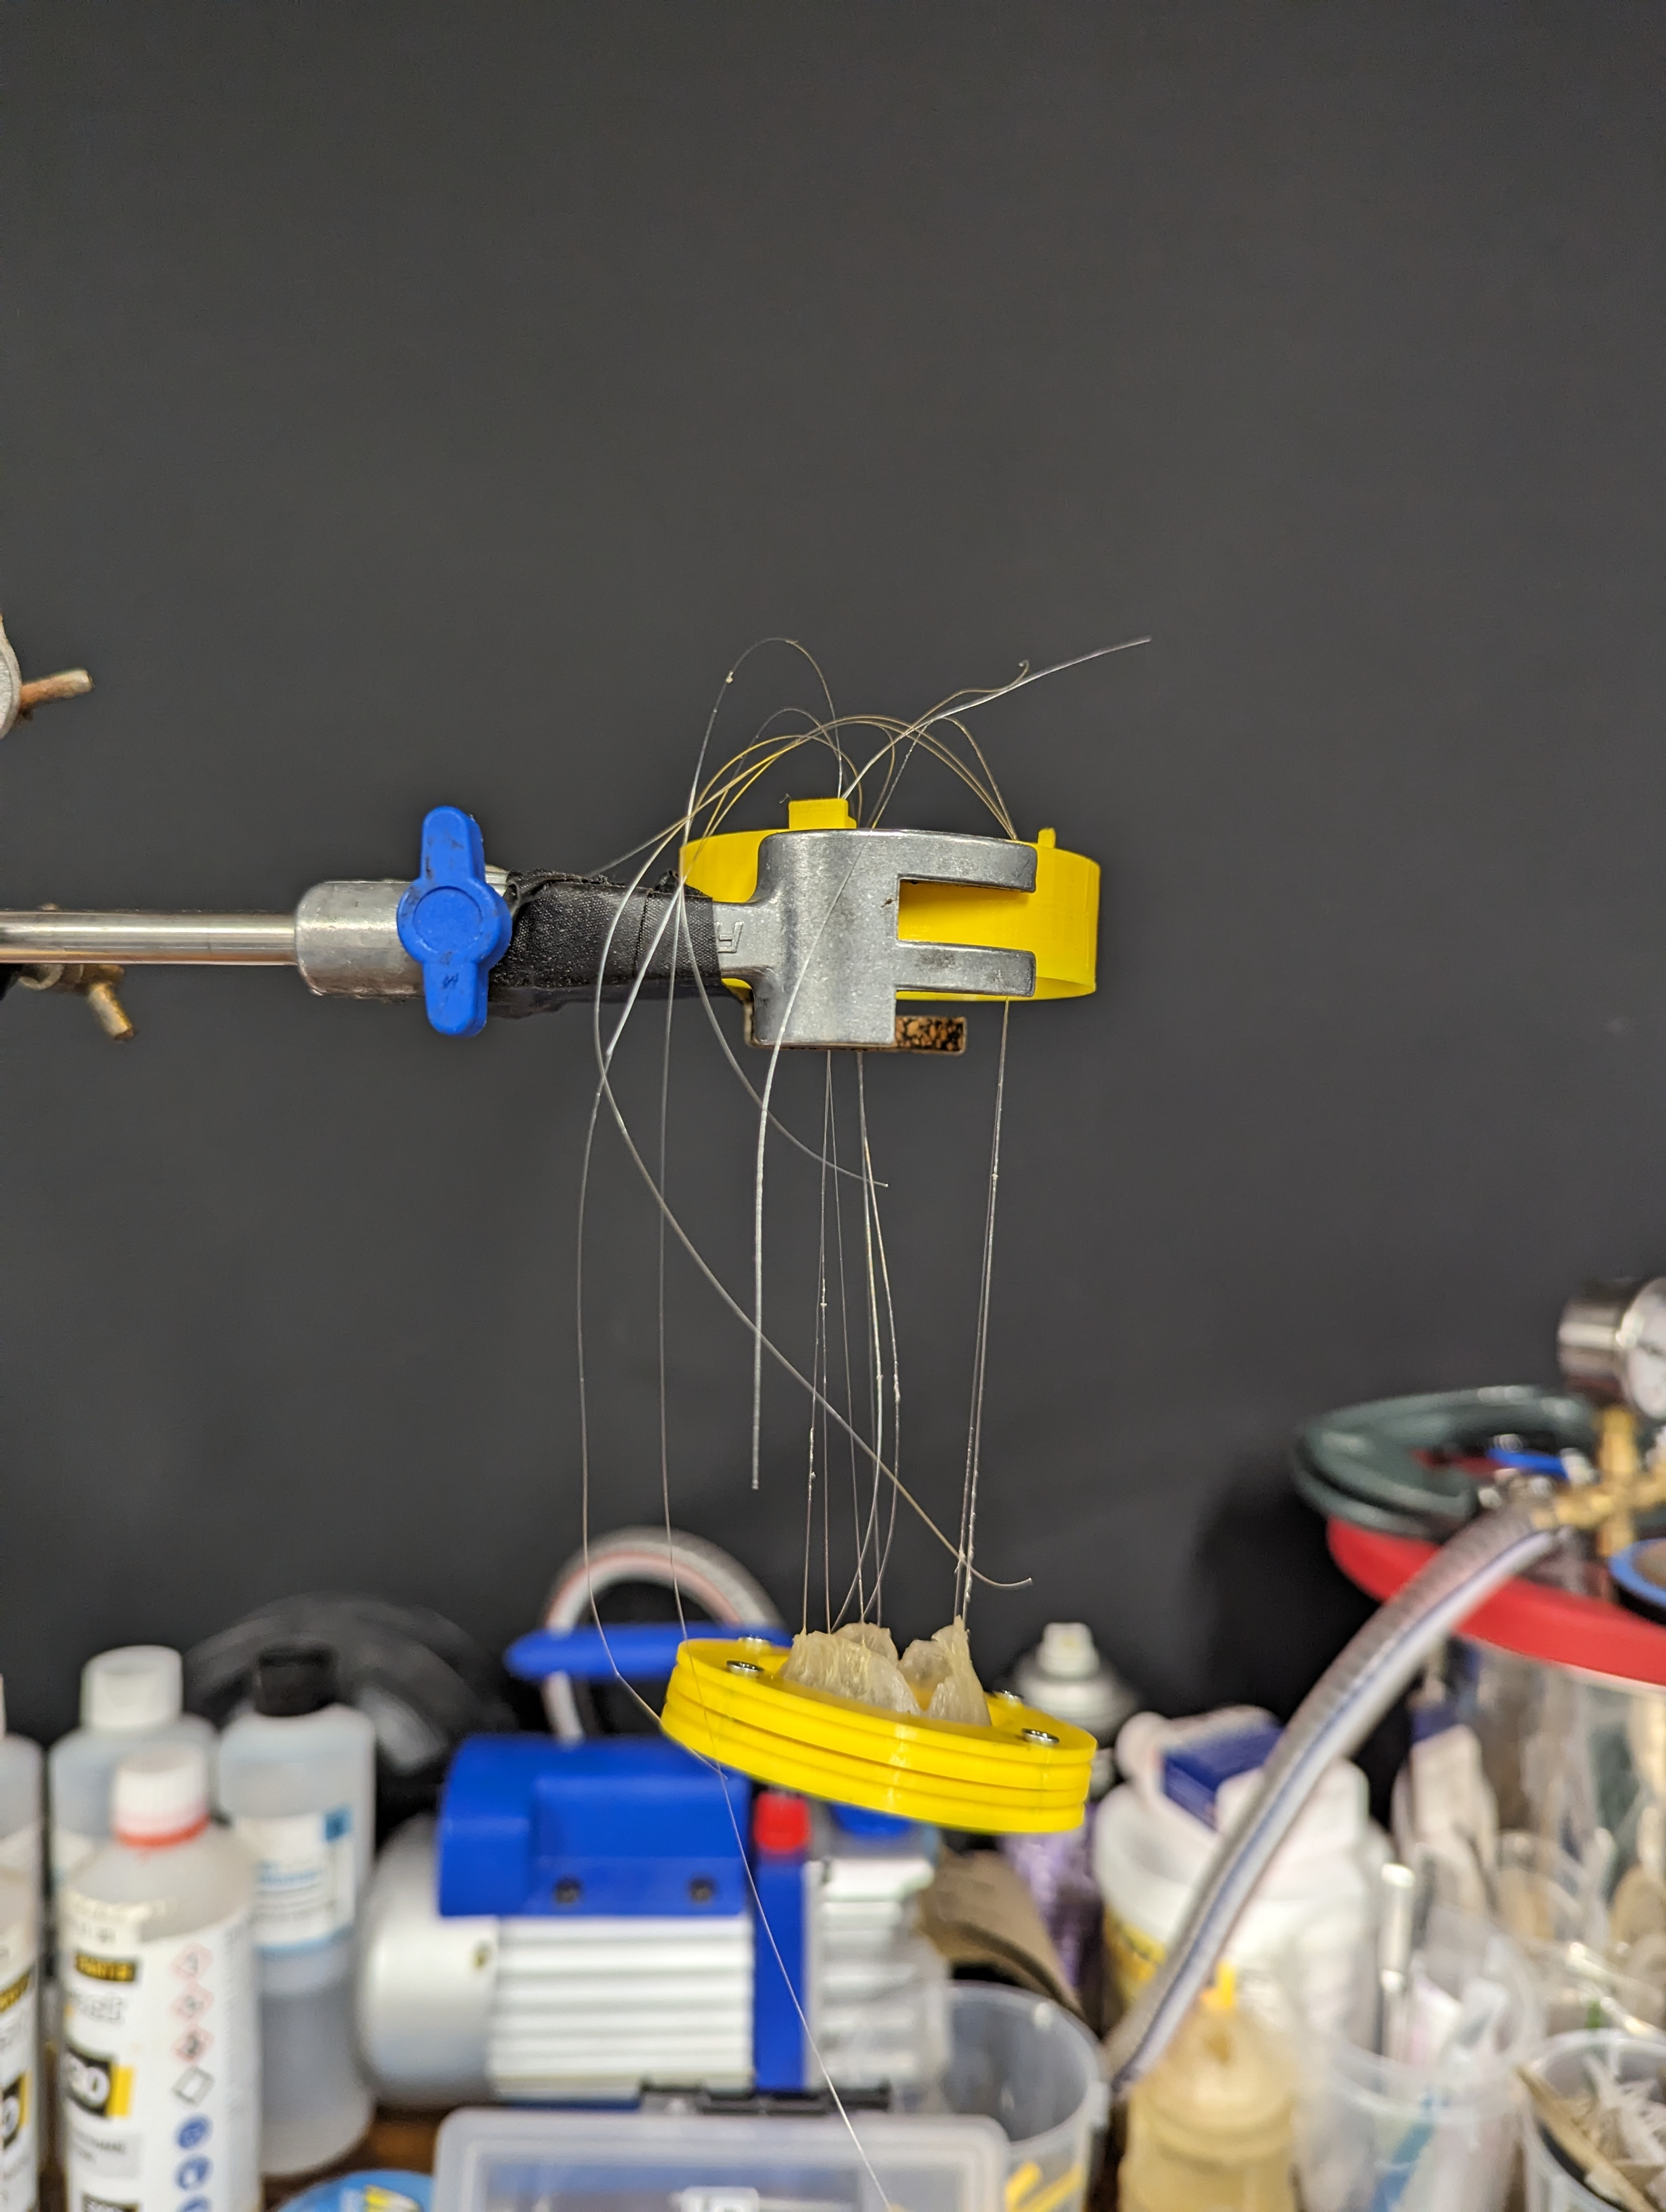
\includegraphics[width=0.8\textwidth]{figures/assemblingfixtures.jpg}
    \caption{Tensioning of chordae tendineae}
    \label{fig:chordtens}
\end{figure}
\section{Rig Assembly}

Once the core testing aparatus was assembled, the various adapters for routing the pulsatile flow loop to the valve and valve to reservoir were wrapped in teflon tape to secure the connections from leaks.

When all connections were securely tightened, the components were levelled to eye with pads of styrofoam.

\section{Testing Procedure}

\subsection{Pilot Checks}
Prior to the main testing a series of system leakage checks were performed to ensure minimal leaking throughout the main tests. Leakage in coaptation testing results in a great loss in the differential pressure across the valve resulting in a reduced coaptation for the same pump displacement.

The reservoir was filled and leur lock valve on the pulsatile pumped was opened so the system could fill with fluid. The system was then purged of air bubbles by using a guide wire and syringe to pull the air out. As leakage spots were observed they were sealed with blue tack.
\begin{figure}
    \centering
    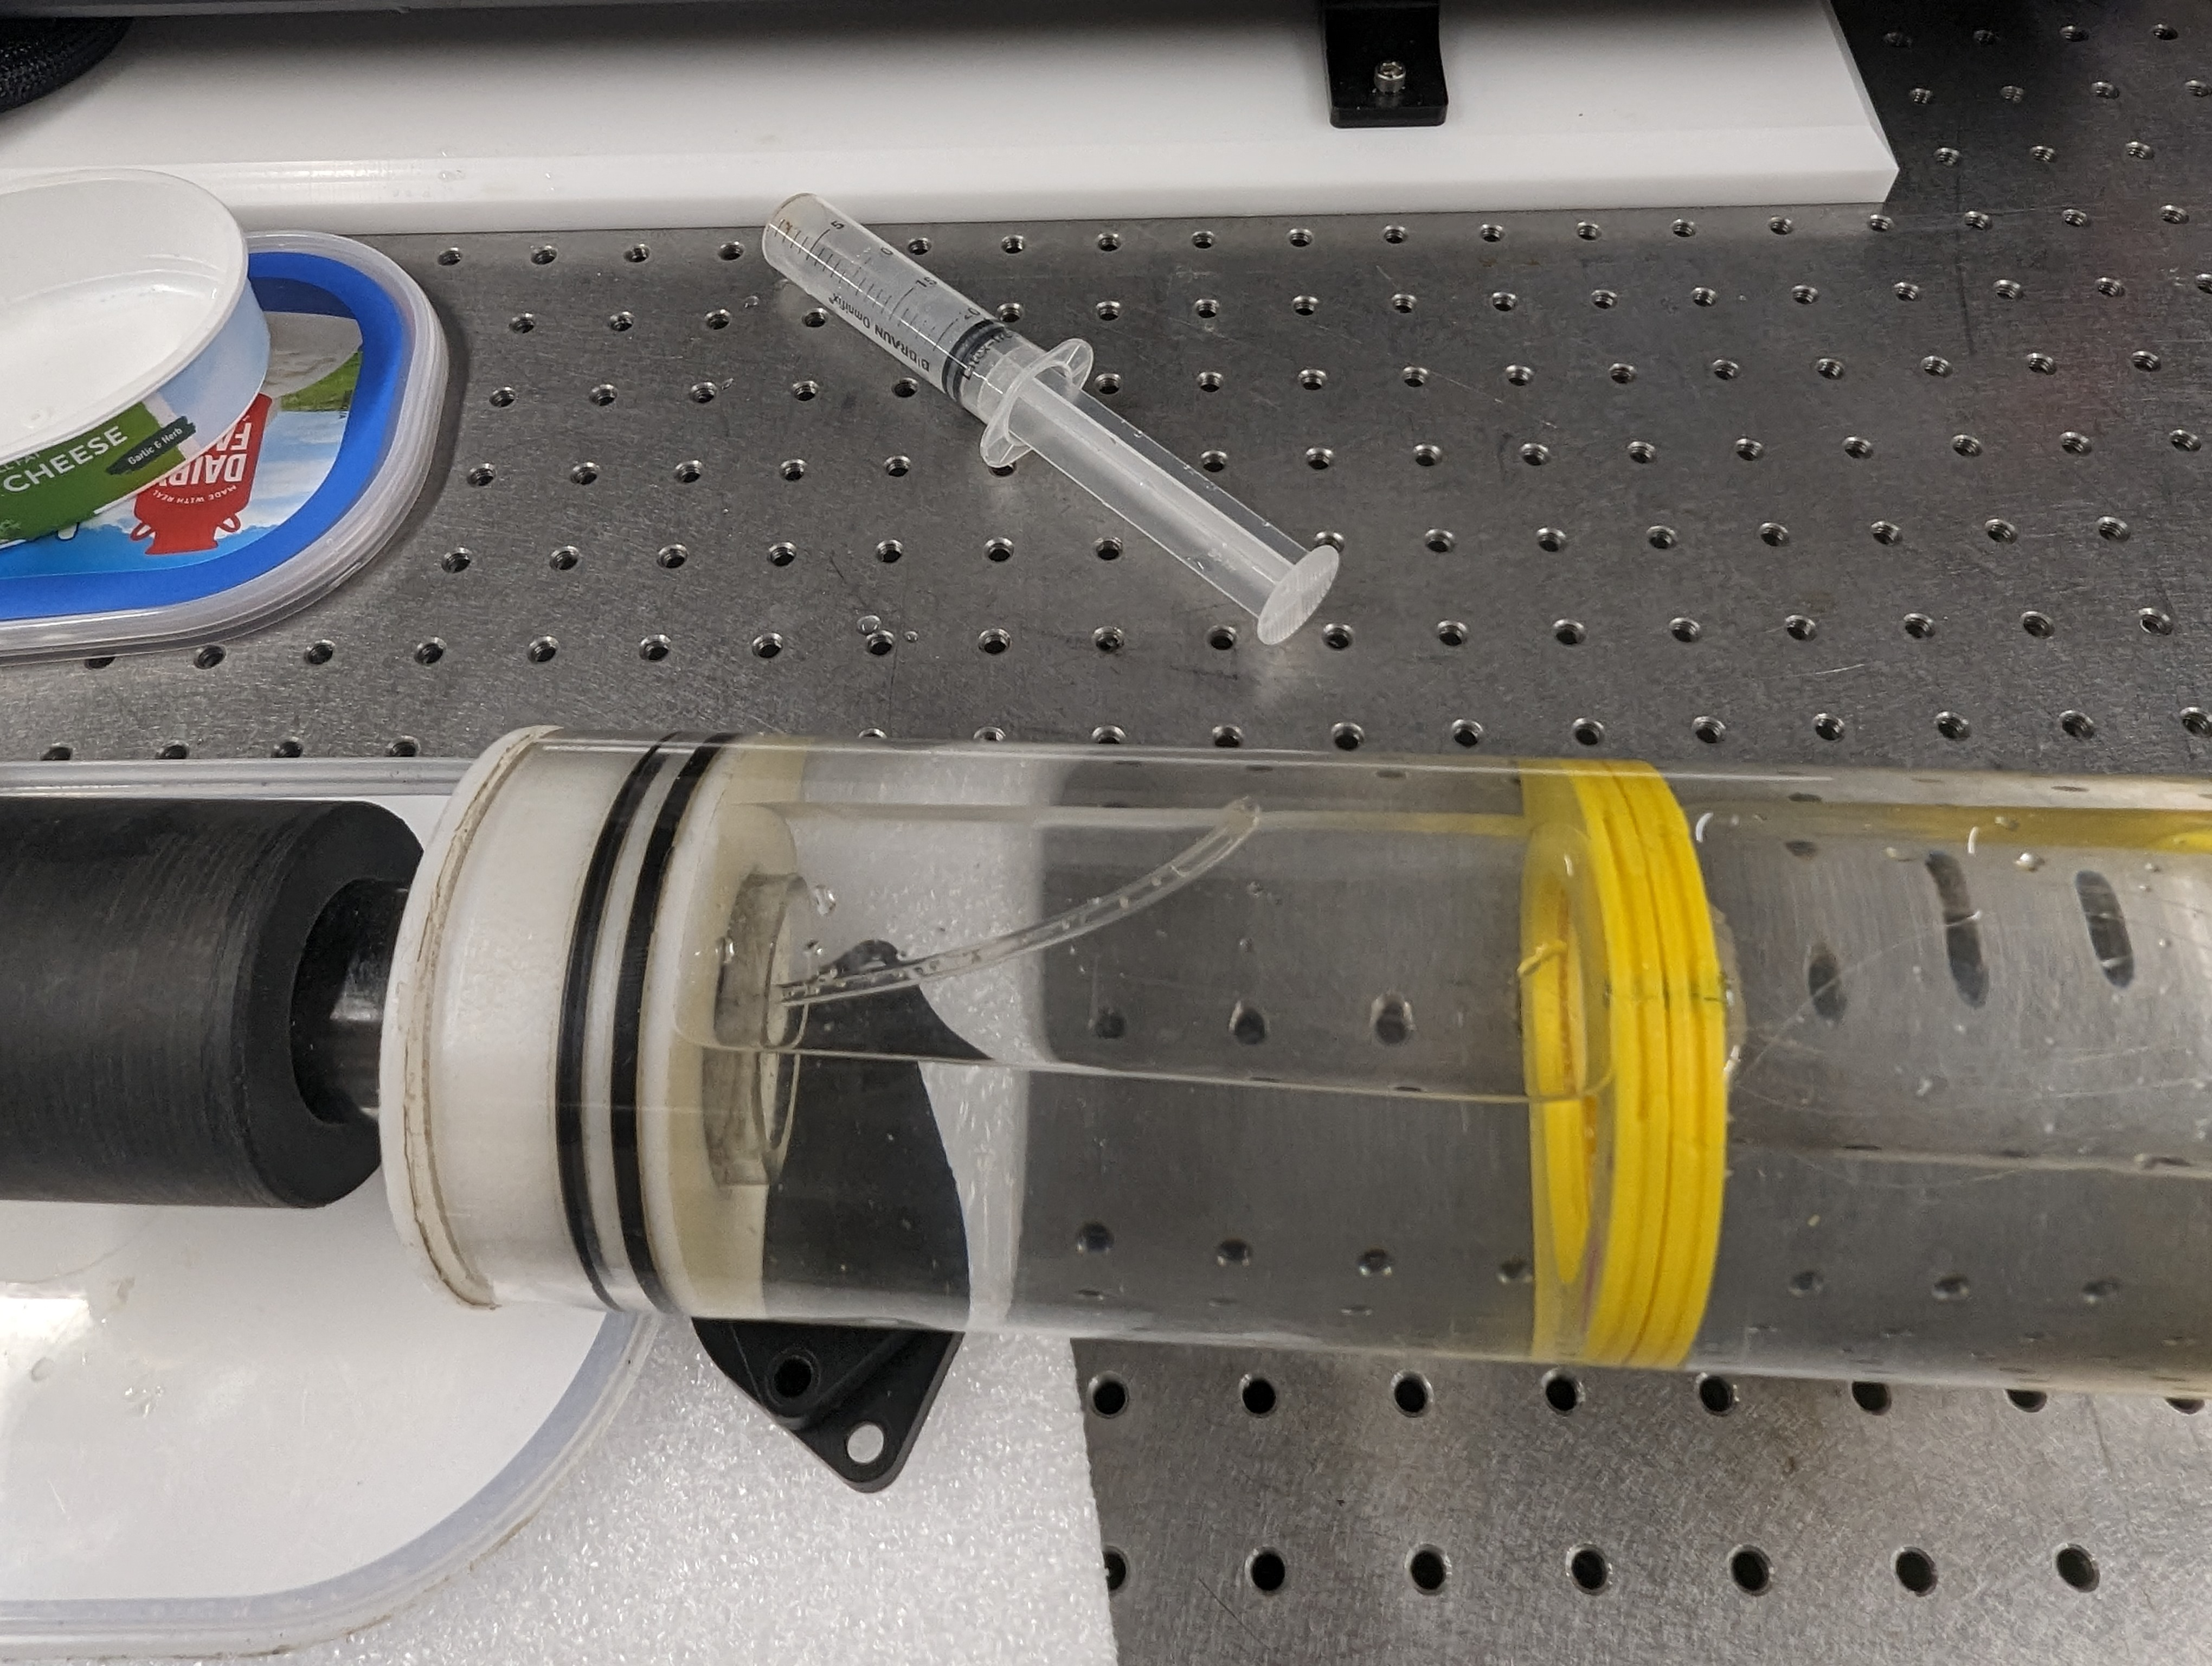
\includegraphics[width=0.8\textwidth]{figures/suckingoutbubbles.jpg}
    \caption{Removing air bubbles from the system}
    \label{fig:leakcheck}
\end{figure}

\subsection{Coaptation Testing}
Once leaks were adequately sealed and air bubbles removed, the pulsatile flow loop was started. The pulsatile pump had a set displacement and frequency.
This was sequenced to remove new bubbles which the system leaks introduced as the testing progressed which obscured the visual and performance of the valve.
The valve was observed and recorded for coaptation at multiple angles.
To see if the valve presented failure from cyclic stress at the chordae tendineae attachments the test was let to run for 10 minutes.
\begin{figure}
    \centering
    \includegraphics[width=0.8\textwidth]{figures/testrigbirdseye.jpg}
    \caption{Birds eye view of the test rig}
    \label{fig:rig}
\end{figure}
\todo{change to subfloats}
% \section{Challenges and Mitigations}

% \begin{itemize}
%   \item Leakage: The pulsatile flow loop is a closed system, so leakage has to be carefully monitored. With the nature of the proof of concept rig containing many adapters and connections, it is important to ensure that all connections are secure and that there are no leaks.
%         \begin{itemize}
%           \item Mitigation: This was managed with the liberal use of teflon tape and tight fit Buna O-rings. Where there were still leaks, small containers was used to catch the fluid and pour back into the circuit.
%         \end{itemize}
%   \item Air bubbles: Air bubbles greatly obstructed the coaptation of the valve leaflets. Interupting the fluid flow and also obscuring the view of the valve for evaluation of the coaptation.
%         \begin{itemize}
%           \item Mitigation: With the leaks in the system allowing air to enter repeated purging of the system was required to remove air bubbles with a syringe and tube entering through the proximal end of the system.
%         \end{itemize}
%   \item Chordae Tendineae Adhesion: The adhesion of the most recently attached mock tendineae to the \gls{PU} leaflets had not fully set before the testing began. This resulted in the one of the tendineae detaching during coaptation.
%         \begin{itemize}
%           \item Mitigation: As the valve was still functioning the testing was not stopped to mitigate this issue.
%         \end{itemize}
% \end{itemize}
